Automated drilling will most likely involve linking downhole and surface measurements with real-time models to improve the safety and efficiency of the drilling process. The main idea is that downhole and surface sensors will communicate measurements to a computer which in turn will display and process the data, as well as control drilling parameters. A computer algorithm will then control that the operation is safe and try to optimize the drilling efficiency by adjusting a set of controllable parameters. The only manual control will be the START button, which means that when drilling has started, no additional manual intervention should be required.

\numberwithin{equation}{section}
\numberwithin{figure}{section}
\numberwithin{table}{section}

A safe operating range will be defined for all the monitored parameters and any measurement outside the range will cause the control system to reduce the RPM and WOB, lift the drill string off-bottom or shut down the system depending on how critical the situation is. The value of the different limits will be based on both equipment specifications and experimental work.

To ensure the efficiency of the operation, an optimization function will be defined. It will seek to improve the drilling efficiency while ensuring the safety of the personnel and equipment. By continuously adjusting the control parameters and monitoring their response, the algorithm will aim to optimize the drilling operation. In this case, the control parameters will be the WOB, RPM and the pump flow rate, and the response parameters will be the torque, ROP, vibration amplitude, inclination and azimuth, temperature and pressure. 

\begin{figure} [H]
\centering
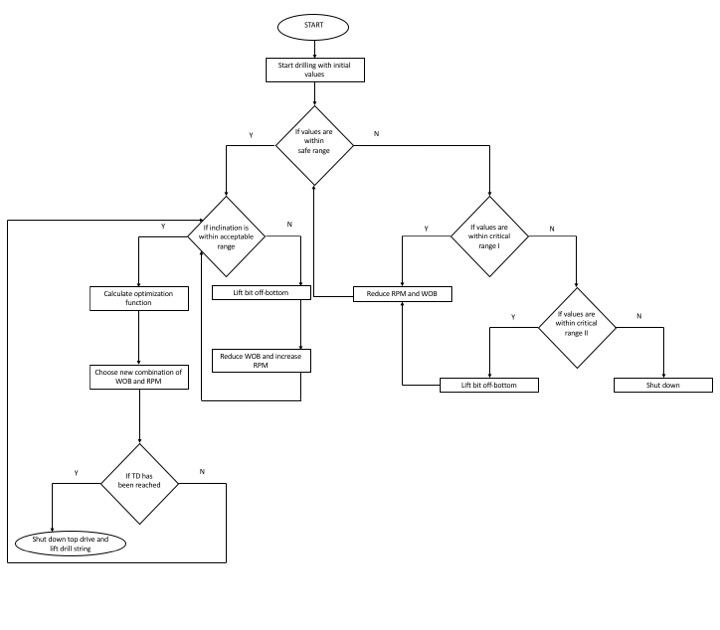
\includegraphics[width=1.0\textwidth]{figures/GeneralAlg.jpg}
\caption{Flow chart illustrating the general control algorithm}
\label{fig:algoflowchart}
\end{figure}


Figure (\ref{fig:algoflowchart}) shows how the drilling algorithm works step by step. When pressing the START button, the initial values for the control parameters are set, and drilling and continuous monitoring of key parameters start. The next step is to ensure that all parameters are within the safe operating range. If they are not, the algorithm will respond. If parameters are within the safe range, drilling continues and optimization can start. 

The purpose of the optimization function is to choose the best combination of control parameters to maximize the efficiency of the drilling operation. This procedure will continue until the desired depth has been reached. 

A way to monitor drilling efficiency is to measure the speed of drilling, or in other terms, the Rate of Penetration (ROP). ROP is a measure of depth drilled per unit time and maximizing this value will be crucial in carrying out an efficient drilling operation. 

\subsection{Drilling Optimization}
Maximizing ROP can be treated as an optimization problem. The goal of optimization is to maximize or minimize a given function by systematically choosing input values and calculating the value of the function. In more general terms, optimization is finding the best available value of a function given a defined domain. Applying the theory of mathematical optimization to this case, the goal will be to find the best available value of WOB and RPM to generate the highest possible ROP. The first step in this problem will be to define an optimization function.

There are different possible optimization functions, one of them is the concept of Mechanical Specific Energy. The function relates WOB, RPM, ROP and torque, and is a measure of how much energy is required to remove a unit volume of rock. Minimizing MSE is one way to maximize the ROP and consequently, the drilling efficiency. 

Another approach is to define a function which quantifies the amount of energy wasted in the system. It would be a function of the vibrations in the drill string as these are expected to be the largest cause of energy loss. Minimizing the energy waste would result in maximizing the useful energy and, thus, maximizing the drilling efficiency.

A third approach is to combine the two concepts introduced above. Such a function would improve drilling efficiency both by ensuring the least possible amount of energy is needed to remove the rock and by reducing the amount of energy wasted.

A further introduction to drilling optimization will be given to provide a deeper understanding of the choice of optimization function and algorithm.

\subsubsection{MSE Minimization}

A possible optimization function that can be used in this case is the function of Mechanical Specific Energy which is a measure of how much energy is required to remove a unit volume of rock and it is usually expressed in terms of drilling parameters such as weight on bit (WOB), torque, rate of penetration (ROP) and rotational speed (RPM). Choosing the optimum combination of controllable variables to minimize the MSE, will result in optimizing the drilling efficiency. 

MSE is defined by equation (\ref{eq:mse}).

\begin{equation}
\centering
   MSE = \frac{Total Energy Input}{Volume Removed}
\label{eq:mse}
\end{equation}

There are two forces acting on the bit during drilling: WOB (axial force) and torque (rotational force). MSE can be expressed in terms of these forces, as shown in equation (\ref{eq:msev}) and (\ref{eq:mset}). 

\begin{equation}
\centering
   MSE = \frac{Vertical Energy Input}{Volume Removed} + \frac{Rotational Energy Input}{Volume Removed}
\label{eq:msev}
\end{equation}

\begin{equation}
\centering
   MSE = \frac{WOB x \Delta h}{Area x \Delta h} + \frac{Torque x 2\pi x Numbers of rotations}{Volume Removed}
\label{eq:mset}
\end{equation}

Because the distance travelled by the bit is the ROP divided by the RPM, equation (\ref{eq:mset}) can be rearranged to give equation (\ref{eq:mser}).

\begin{equation}
\centering
   MSE = \frac{WOB}{Area} + \frac{2\pi x RPM x Torque}{Area x ROP}
\label{eq:mser}
\end{equation}

As shown in equation (\ref{eq:mser}), MSE is a function of drilling parameters that will be monitored continuously through the drilling process. Using MSE as an optimizing function is therefore a possible solution to ensuring an effective drilling operation. 

However, an important factor to consider is that MSE is not only a function of drilling efficiency, it is also a function of the type of rock that is being drilled through.

Instead of choosing WOB and RPM combinations randomly, experiments can be done to define a few regimes that will work well in the most common formations. This will be done to avoid trying out combinations that are unlikely to have good results. It is important to note that this is not a way to identify rock types, it is a way to make a better initial guess for the optimization algorithm.

A few different rock types will be selected based on what is most likely to encounter when drilling a well and they will have very different properties to cover a wider range of possibilities. Test drilling will then be performed to determine the best ranges of WOB and RPM for the different rock types. These ranges of values will be the main area where the algorithm looks for a good combination of control parameters. The tests will be conducted once the rig has been constructed and the system is ready to be tested.

\subsubsection{Vibration Minimization}

A second way to optimize the drilling efficiency is to minimize the waste of energy. When drilling, the goal is that all the energy provided by the top drive should be used to remove rock. However, a lot of the energy transforms into vibrations. To ensure that the operation is as efficient as possible, the goal will be to minimize the waste of energy.

Vibrational motion can be understood in terms of the conservation of energy. When the pipe is displaced from its center, some potential energy is stored in the pipe. When it is released and returns to its neutral state, its mass is accelerated and the potential energy is transformed into kinetic energy. The mass then decelerates and transfers the kinetic energy back to its potential. Oscillation of the drill string therefore amounts to transferring back and forth from kinetic energy to potential energy.

To quantify the amplitude of the vibrations, the amount of energy in the oscillation can be calculated. By using an accelerometer downhole, continuous measurements of the movement can be made and this will enable the calculation of the waste of energy through vibrations. 

The waste of energy can then be minimized by creating an optimization algorithm that uses the accelerometer measurements to monitor the vibration energy, and the control parameters to reduce the vibration amplitude.

\subsubsection{Borehole Verticality}

One of the main requirements of the rig is to be able to drill as vertically as possible which will be ensured by downhole sensors. A gyroscope and an accelerometer will be included in the same sensor and, although they are similar in purpose, they measure different things and together they provide accurate information about position and orientation.

The expected cause behind deviation is the occurrence of a tilted layer or encountering a new layer/rock inclusion with different rock properties. This may cause the bit to deviate from vertical position as it attempts to find the easiest path to drill.

To include a response to a change in inclination in the optimization function, a range of acceptable inclination values must be defined. This means that if the change in inclination is larger than a given value, the control system will respond by lifting the bit a pre-defined length and resume drilling with lower WOB and the same or higher RPM.


\subsection{Algorithm for finding Global Maximum of Optimization Function}

As explained previously, the aim of the model is to continuously ensure the safety of the equipment and personnel, as well as improve drilling efficiency by using an optimization algorithm. There are several optimization methods that can be used in this situation and a review of three different possibilities will be provided below.

\subsubsection{Gradient Descent and Gradient Ascent}

The Gradient Descent method, also known as Steepest Descent, is a first order iterative optimization algorithm. Given a function defined by different sets of parameters, the Gradient Descent method starts with a set of initial parameter values. By solving the problem iteratively, for each step of iteration a new set of variables is chosen and we move towards a minimum point to minimize the given function. In other words, we take steps proportional to the negative of the gradient. 

Gradient Descent is an algorithm used to find the nearest minimum point. Gradient Ascent is the opposite. The same procedure is used, but in this case, the nearest maximum is approached by moving proportionally to the positive of the gradient. This a sort of Hill Climbing solution method. 

Gradient Descent and Gradient Ascent are excellent choices if there is only one maximum or minimum point. In this problem, the number of maximum or minimum points is unknown. 
Both Gradient Descent and Gradient Ascent use local searches and the risk of getting stuck in a local optimum or minimum is therefore large. This means that the algorithm is tricking us to believe the given set of variables is the best solution to optimize the drilling operation. In reality, there exists a set of other parameters that may lead to better drilling performance. Our main goal is to optimize the drilling operation without getting stuck in a local maximum or minimum and try to find the global maximum or minimum, the gradient descent/ascent method is therefore not the optimal choice.


\begin{figure} [H]
\centering
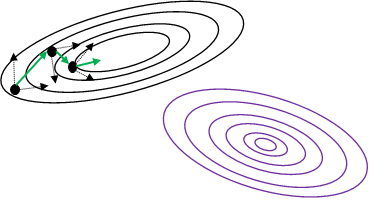
\includegraphics[width=0.7\textwidth]{figures/gradientdescentmethod.png}
\caption{Illustration of the gradient descent method}
\label{fig:gradientdm}
\end{figure}

As illustrated in figure (\ref{fig:gradientdm}), the Gradient Ascent method uses a local search to find the optimum point of the function. The risk is that it finds a local optimum, black circles, instead of a global optimum, purple circles.

\subsubsection{Simulated Annealing}

Simulated Annealing (SA) is a probabilistic method to estimate the global maximum of a given problem. The method uses the same approach as Hill Climbing, but it occasionally selects random sets of variables and allows the algorithm to use solutions that are worse than the current. By doing this, the algorithm avoids a premature convergence which occurs when the algorithm thinks the chosen variables are optimal (stuck in a local optimum), but the solution is actually a suboptimal. 

Compared to the method of gradient descent/ascent, this method eliminates the risk of getting stuck in a local optimum point which is positive. However, it allows using solutions that are worse than the current one which might cause the method to be less effective than the steepest descent. The benefit of reaching a global optimum versus only a local optimum should be compared to the drawback of spending time drilling in a regime that is worse than the current one.

Figure (\ref{fig:siman}) illustrates how the Simulated Annealing algorithm chooses random sets of variables (x1, x2, x3…) to determine the location of the global maximum and how it allows using solutions that are worse than the current one (x4 and x5 vs x3).

\begin{figure} [H]
\centering
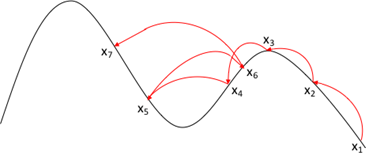
\includegraphics[width=1.0\textwidth]{figures/siman.png}
\caption{Illustration of the simulated annealing method}
\label{fig:siman}
\end{figure}

\subsubsection{Genetic Algorithms}

Genetic Algorithms (GA) is a method inspired by Charles Darwin’s Theory of Natural Selection and is used to solve both constrained and unconstrained optimization problems. Genetic Algorithms start with randomly selected variables in the initial generation of candidate solutions that are tested against the objective function. From the initial generation, the best performing variables are favored and selected to reproduce. 

There are two possible outcomes for the next generation. The first one is called a crossover and involves two favorable variables from the previous generation combining to create a new generation of population. The previous generation can be referred to as parents and the new one as children. 

The second one is called a mutation. Here, one favorable parent from the previous generation is combined with one favorable child from the current generation to create an individual for the new generation. Using mutations helps to find the global optimum point and avoids the risk of the algorithm getting stuck in a local optimum. 

For each new generation, individuals that are evolving towards an optimal solution of the function will be used as parents for the next generation. This process continues until the desired optimization is established. 

Figure (\ref{fig:genetic}) shows the evolution of the different generations and how the algorithm differentiates between local optimums (blue circles) and the global optimum (red circles). The favorable variables, the ones closest to a local or global optimum, are shown as colored triangles and the desired optimum is the black triangle.

\begin{figure} [H]
\centering
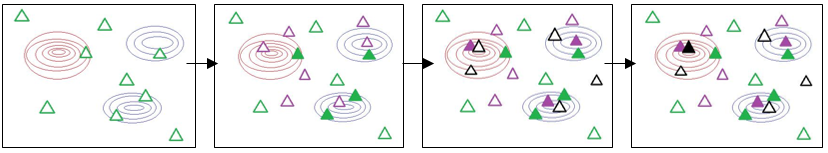
\includegraphics[width=1\textwidth]{figures/genetic.PNG}
\caption{Illustration of the concept of genetic algorithms}
\label{fig:genetic}
\end{figure}


The benefit of using a Genetic Algorithm is that the risk of getting stuck in a local optimum point is eliminated. The problem is that it requires trying out many different combinations of parameters for every generation of solutions and this may be too time-consuming for a small-scale drilling operation.

\subsubsection{Proposed Solution}

The Gradient Descent method will not be used because the risk of getting stuck in a local optimum point is large compared to the other two methods. Both the Genetic and Simulated Annealing methods are good choices, but they are time consuming since they must test many control parameter combinations before selecting the optimum solution. The main difference between the two methods is that the Genetic Algorithms will test several combinations before moving to the next step, while Simulated Annealing will test one combination for each step. Because many different rock types may be encountered when drilling, the range of the control parameters is expected to be large and the Genetic Algorithm is therefore preferred.

To solve this optimization problem, the Genetic Algorithm method has been chosen, but it has been simplified in order to save time. The optimization function will be a combination of MSE and vibration energy, and the aim will be to minimize it.

\begin{figure} [H]
\centering
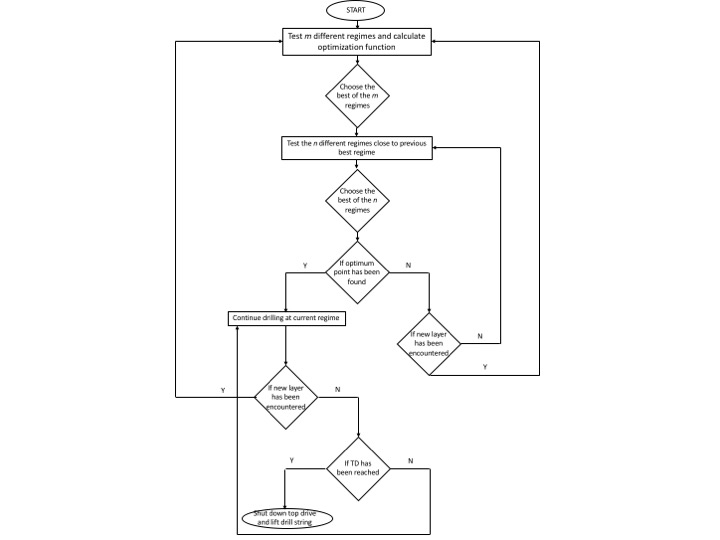
\includegraphics[width=1.0\textwidth]{figures/OptAlg.jpg}
\caption{Flow chart of the optimization algorithm}
\label{fig:optialgo}
\end{figure}

The first step is to choose m combinations of input values within the range of data determined from the testing of rock samples. Drilling will continue at the regime that resulted in the optimum value for the optimization function. Next, the search range is reduced and moved close to the previous best solution. n new combinations of parameters are tested and drilling continues with the best combination. 

A criterion to determine whether the drilling efficiency is satisfactory must be defined. A possibility is to use MSE. When the difference between the MSE at the previous regime and the MSE at the current regime is small enough, the control parameters can be assumed to be optimal. The critical value y will be determined during the testing phase. This combination of parameters will be used until a new layer is reached.

A possible way to identify a new layer is to monitor how much the ROP changes. When the change in ROP is sudden and large, it may be assumed that a new layer is encountered and the optimization process must start again from the first step.

The algorithm is illustrated in figure (\ref{fig:optialgo}).

In this year’s competition, a pilot hole will be pre-drilled using the same bit as the on-site test and must be less than 1 in deep. This will not require any optimization, so a simpler version of the drilling algorithm will be used, as shown in figure (\ref{fig:pilothole}).

\begin{figure} [H]
\centering
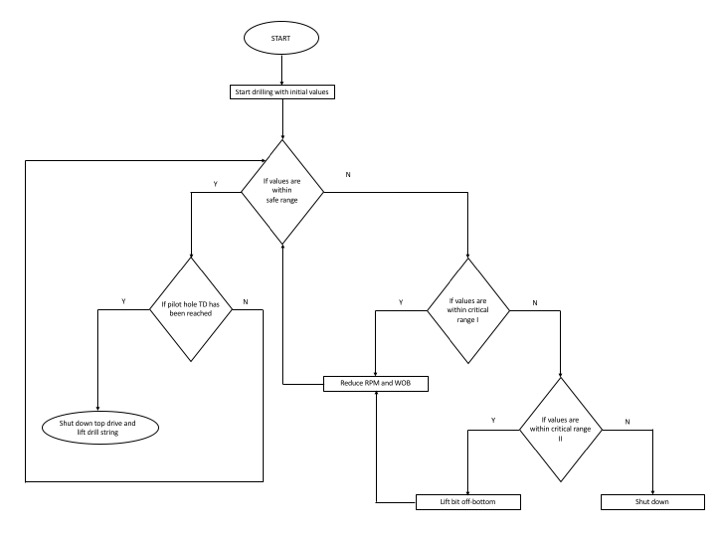
\includegraphics[width=1.0\textwidth]{figures/PilotHole.jpg}
\caption{Flow chart for the pilot hole algorithm}
\label{fig:pilothole}
\end{figure}










